\documentclass[conference]{IEEEtran}
\IEEEoverridecommandlockouts
% The preceding line is only needed to identify funding in the first footnote. If that is unneeded, please comment it out.
%Template version as of 6/27/2024

\usepackage{cite}
\usepackage{amsmath,amssymb,amsfonts}
\usepackage{algorithmic}
\usepackage{graphicx}
\usepackage{textcomp}
\usepackage{xcolor}
\def\BibTeX{{\rm B\kern-.05em{\sc i\kern-.025em b}\kern-.08em
    T\kern-.1667em\lower.7ex\hbox{E}\kern-.125emX}}
\begin{document}

\title{Multi-View Convolutional Neural Network for Musculoskeletal Disorder Detection in Radiographic Imaging*\\
}

\author{\IEEEauthorblockN{1\textsuperscript{st} Camille Trouvé}
\IEEEauthorblockA{\textit{Ecole du Numérique (EDN)} \\
\textit{Faculty of Management, Economy and Science (FGES)}\\
Lille, France \\
trouve.camille@gmail.com}
\and
\IEEEauthorblockN{2\textsuperscript{nd} Ceren DINC}
\IEEEauthorblockA{\textit{Ecole du Numérique (EDN)} \\
\textit{Faculty of Management, Economy and Science (FGES)}\\
Lille, France \\
cdinc60@gmail.com}
\and
\IEEEauthorblockN{3\textsuperscript{rd} Esteban BOULANGER}
\IEEEauthorblockA{\textit{Ecole du Numérique (EDN)} \\
\textit{Faculty of Management, Economy and Science (FGES)}\\
Lille, France \\
es.boulanger@orange.fr}
\and
\IEEEauthorblockN{4\textsuperscript{th} Roger ACHKAR, Ph.D}
\IEEEauthorblockA{\textit{Faculty of Engineering & Technology} \\
\textit{Antonine University}\\
Baabda, Lebanon \\
dean.fet@ua.edu.lb }
}

\maketitle

\begin{abstract}
Musculoskeletal disorders are among the main causes of disability, according to the World Health Organization. This study aims to develop a tool capable of determining abnormalities in musculoskeletal radiographs. The proposed model is a convolutional neural network based on ResNet18 architecture with a multiple-view fusion module to integrate multiple radiographic projections, mimicking how radiologists interpret radiographic views. The model was trained and tested on the MURA dataset (Stanford), a large open-access dataset combining 40,561 radiographic images of the upper extremity from multiple studies. Through systematic evaluation of seven experimental configurations, the best-performing model achieved a validation AUC-ROC of 0.6545, representing a substantial improvement of +0.0906 compared to the baseline.
\end{abstract}

\begin{IEEEkeywords}
Musculoskeletal disorders, Radiography, Deep learning, CNN, Multi-view fusion
\end{IEEEkeywords}

\section{Introduction}
Musculoskeletal conditions represent a profound global health challenge, affecting approximately 1.7 billion people and serving as the primary driver of disability worldwide\cite{rajpurkar_mura_2018}. These disorders, which include fractures, osteoarthritis, and various degenerative joint diseases, significantly impair mobility and dexterity, often leading to premature exit from the workforce and a diminished quality of life. The increasing prevalence of these conditions, exacerbated by a growing and aging population, has placed an unprecedented strain on healthcare systems\cite{chada_machine_2019}. Radiologists  workloads rise because of a higher volume of complex images, which contributes to fatigue and a statistically significant risk of diagnostic error\cite{rajpurkar_mura_2018,chea_current_2020,singh_hybrid_2022}.

In this context, artificial intelligence (AI), specifically deep learning (DL) utilizing convolutional neural networks (CNNs), has emerged as a tool for diagnostic assistance\cite{chada_machine_2019,chea_current_2020,dangelo_artificial_2022}. CNN architectures are uniquely suited for image-based problems because they can autonomously learn discriminative features from large datasets, matching or even exceeding human performance in narrow tasks\cite{chea_current_2020,singh_hybrid_2022}. Within musculoskeletal radiology, DL applications have expanded across four primary categories: lesion detection, classification, segmentation, and non-interpretive tasks such as protocol optimization. While expert-level performance has been achieved in specific domains like bone age assessment and certain fracture detections, comprehensive interpretation of complex imaging examinations remains an ongoing challenge\cite{chea_current_2020,dangelo_artificial_2022}.

A pivotal milestone in this field was the release of the MURA (Musculoskeletal Radiographs) dataset, a large-scale collection of 40,561 upper extremity images manually labeled by board-certified radiologists\cite{rajpurkar_mura_2018}. Initial benchmark studies using a 169-layer DenseNet achieved high overall AUC-ROC scores but revealed a significant performance gap in specific anatomical regions, particularly the finger and humerus radiographs, where the model struggled to match the agreement levels of practicing radiologists. Furthermore, many existing models operate on single radiographic projections, whereas clinical diagnosis typically necessitates the integration of multiple views to resolve spatial ambiguities\cite{rajpurkar_mura_2018,dangelo_artificial_2022}.

This study proposes a multi-view neural network architecture designed to bridge this gap by mimicking the diagnostic process of human experts. By employing a ResNet18 backbone pretrained on ImageNet\cite{he_deep_2016} and a specialized masked average pooling module, the model integrates features from multiple radiographic views into a singular study-level prediction.


\section{Material and Method}

\subsection{Dataset}

In this project, we used the MURA dataset (Musculoskeletal Radiographs), which contains X-ray images of upper limbs labeled as either normal or abnormal\cite{rajpurkar_mura_2018}. Labels are provided at the study level, meaning that all images belonging to the same patient examination share the same label.

Each study $S_i$ contains between one and four radiographic views:
\begin{equation}
S_i = \{ x_i^{(v)} \}_{v=1}^{n_i}, \quad n_i \in \{1,2,3,4\},
\end{equation}
where $x_i^{(v)}$ denotes the $v$-th image of study $i$. Each study is associated with a binary label $y_i \in \{0,1\}$ indicating whether it is abnormal.

Although the full dataset contains more than 40,000 images, we restricted training to a subset of 1,000 studies to reduce computational cost. The official validation split was used for evaluation.

\subsection{Preprocessing and Data Augmentation}

All images were originally stored as grayscale images and were converted to three channels to match the input format of pretrained convolutional neural networks. Images were resized to $224 \times 224$ pixels.

Pixel intensities were normalized using a fixed mean and standard deviation of $(0.5, 0.5, 0.5)$. During training, simple data augmentation techniques such as random horizontal flips were applied.

Since the number of views per study varies, we padded each study to a maximum of four images and used a binary mask:
\begin{equation}
m_i^{(v)} =
\begin{cases}
1 & \text{if view } v \text{ exists} \\
0 & \text{otherwise}
\end{cases}
\end{equation}
to indicate valid views.

\subsection{Model Architecture}

We implemented a multi-view classification model in which each image is processed independently and then aggregated at the study level.

\subsubsection{Feature Extraction}

Each image is passed through a shared ResNet18 network pretrained on ImageNet\cite{he_deep_2016}. The final classification layer is removed, and the output of the network is a feature vector:
\begin{equation}
h_i^{(v)} = f_{\theta}(x_i^{(v)}) \in \mathbb{R}^{512}.
\end{equation}

\subsubsection{Multi-View Aggregation}

The features of all views belonging to the same study are combined using a masked average pooling operation:
\begin{equation}
z_i = \frac{1}{\sum_{v} m_i^{(v)}} \sum_{v=1}^{4} m_i^{(v)} \, h_i^{(v)}.
\end{equation}

This produces a single feature vector $z_i$ representing the entire study.

\subsubsection{Classification}

The aggregated feature vector is then passed through a two-layer feedforward classifier with ReLU activation and dropout for regularization, followed by a sigmoid activation to obtain the predicted probability of abnormality:
\begin{equation}
\hat{y}_i = \sigma(W_2 \, \text{ReLU}(W_1 z_i + b_1) + b_2),
\end{equation}
where $W_1 \in \mathbb{R}^{256 \times 512}$, $W_2 \in \mathbb{R}^{1 \times 256}$, and dropout with rate 0.3 is applied after the ReLU activation. The final output $\hat{y}_i \in (0,1)$ represents the predicted probability of abnormality.

\subsection{Training Procedure}

To handle class imbalance, we used a weighted binary cross-entropy loss:
\begin{equation}
\mathcal{L} =
- \frac{1}{B} \sum_{i=1}^{B}
\left[
w_{+} y_i \log(\hat{y}_i)
+
w_{-} (1 - y_i) \log(1 - \hat{y}_i)
\right].
\end{equation}

The model was trained using the Adam optimizer\cite{kingma_adam_2017} with a batch size of 4. Learning rates were varied across experiments ($3 \times 10^{-4}$, $1 \times 10^{-3}$, and $3 \times 10^{-3}$) to investigate their impact on model performance.

\subsection{Evaluation Metrics}

Model performance was mainly evaluated using the Area Under the Curve Receiver Operating Characteristic (AUC-ROC). In addition, accuracy, sensitivity, and specificity were computed. For a given decision threshold $\tau$, these metrics are defined as:
\begin{align}
\text{Accuracy} &= \frac{\mathrm{TP} + \mathrm{TN}}{\mathrm{TP} + \mathrm{TN} + \mathrm{FP} + \mathrm{FN}}, \\
\text{Sensitivity} &= \frac{\mathrm{TP}}{\mathrm{TP} + \mathrm{FN}}, \\
\text{Specificity} &= \frac{\mathrm{TN}}{\mathrm{TN} + \mathrm{FP}}.
\end{align}


\section{Results}

\subsection{Experimental setup and evaluation metric}
The proposed multi-view model was evaluated on the official validation split of the MURA dataset using study-level labels (normal vs.\ abnormal). Given the class imbalance commonly encountered in medical imaging, performance was primarily assessed using the validation AUC-ROC, as shown in Figure~\ref{fig:final_metrics} and Figure~\ref{fig:hyperparameter_analysis}. To ensure fair comparison across configurations, all experiments were trained using 10 epochs.

\subsection{Overall comparison of experimental configurations}
Seven experimental configurations were compared by varying the learning rate, batch size, and number of training samples. Performance was summarized using the best validation AUC-ROC achieved during training. The configuration with a reduced learning rate (\textit{low\_lr}) achieved the highest performance, with an AUC-ROC of 0.6545, corresponding to an absolute improvement of +0.0906 compared to the baseline configuration (AUC-ROC = 0.5639). Intermediate improvements were observed for the \textit{low\_data} (AUC-ROC = 0.6076) and \textit{large\_batch} (AUC-ROC = 0.6039) configurations, whereas the \textit{more\_data} configuration underperformed relative to the baseline (AUC-ROC = 0.5409).

\begin{figure}[h]
\centering
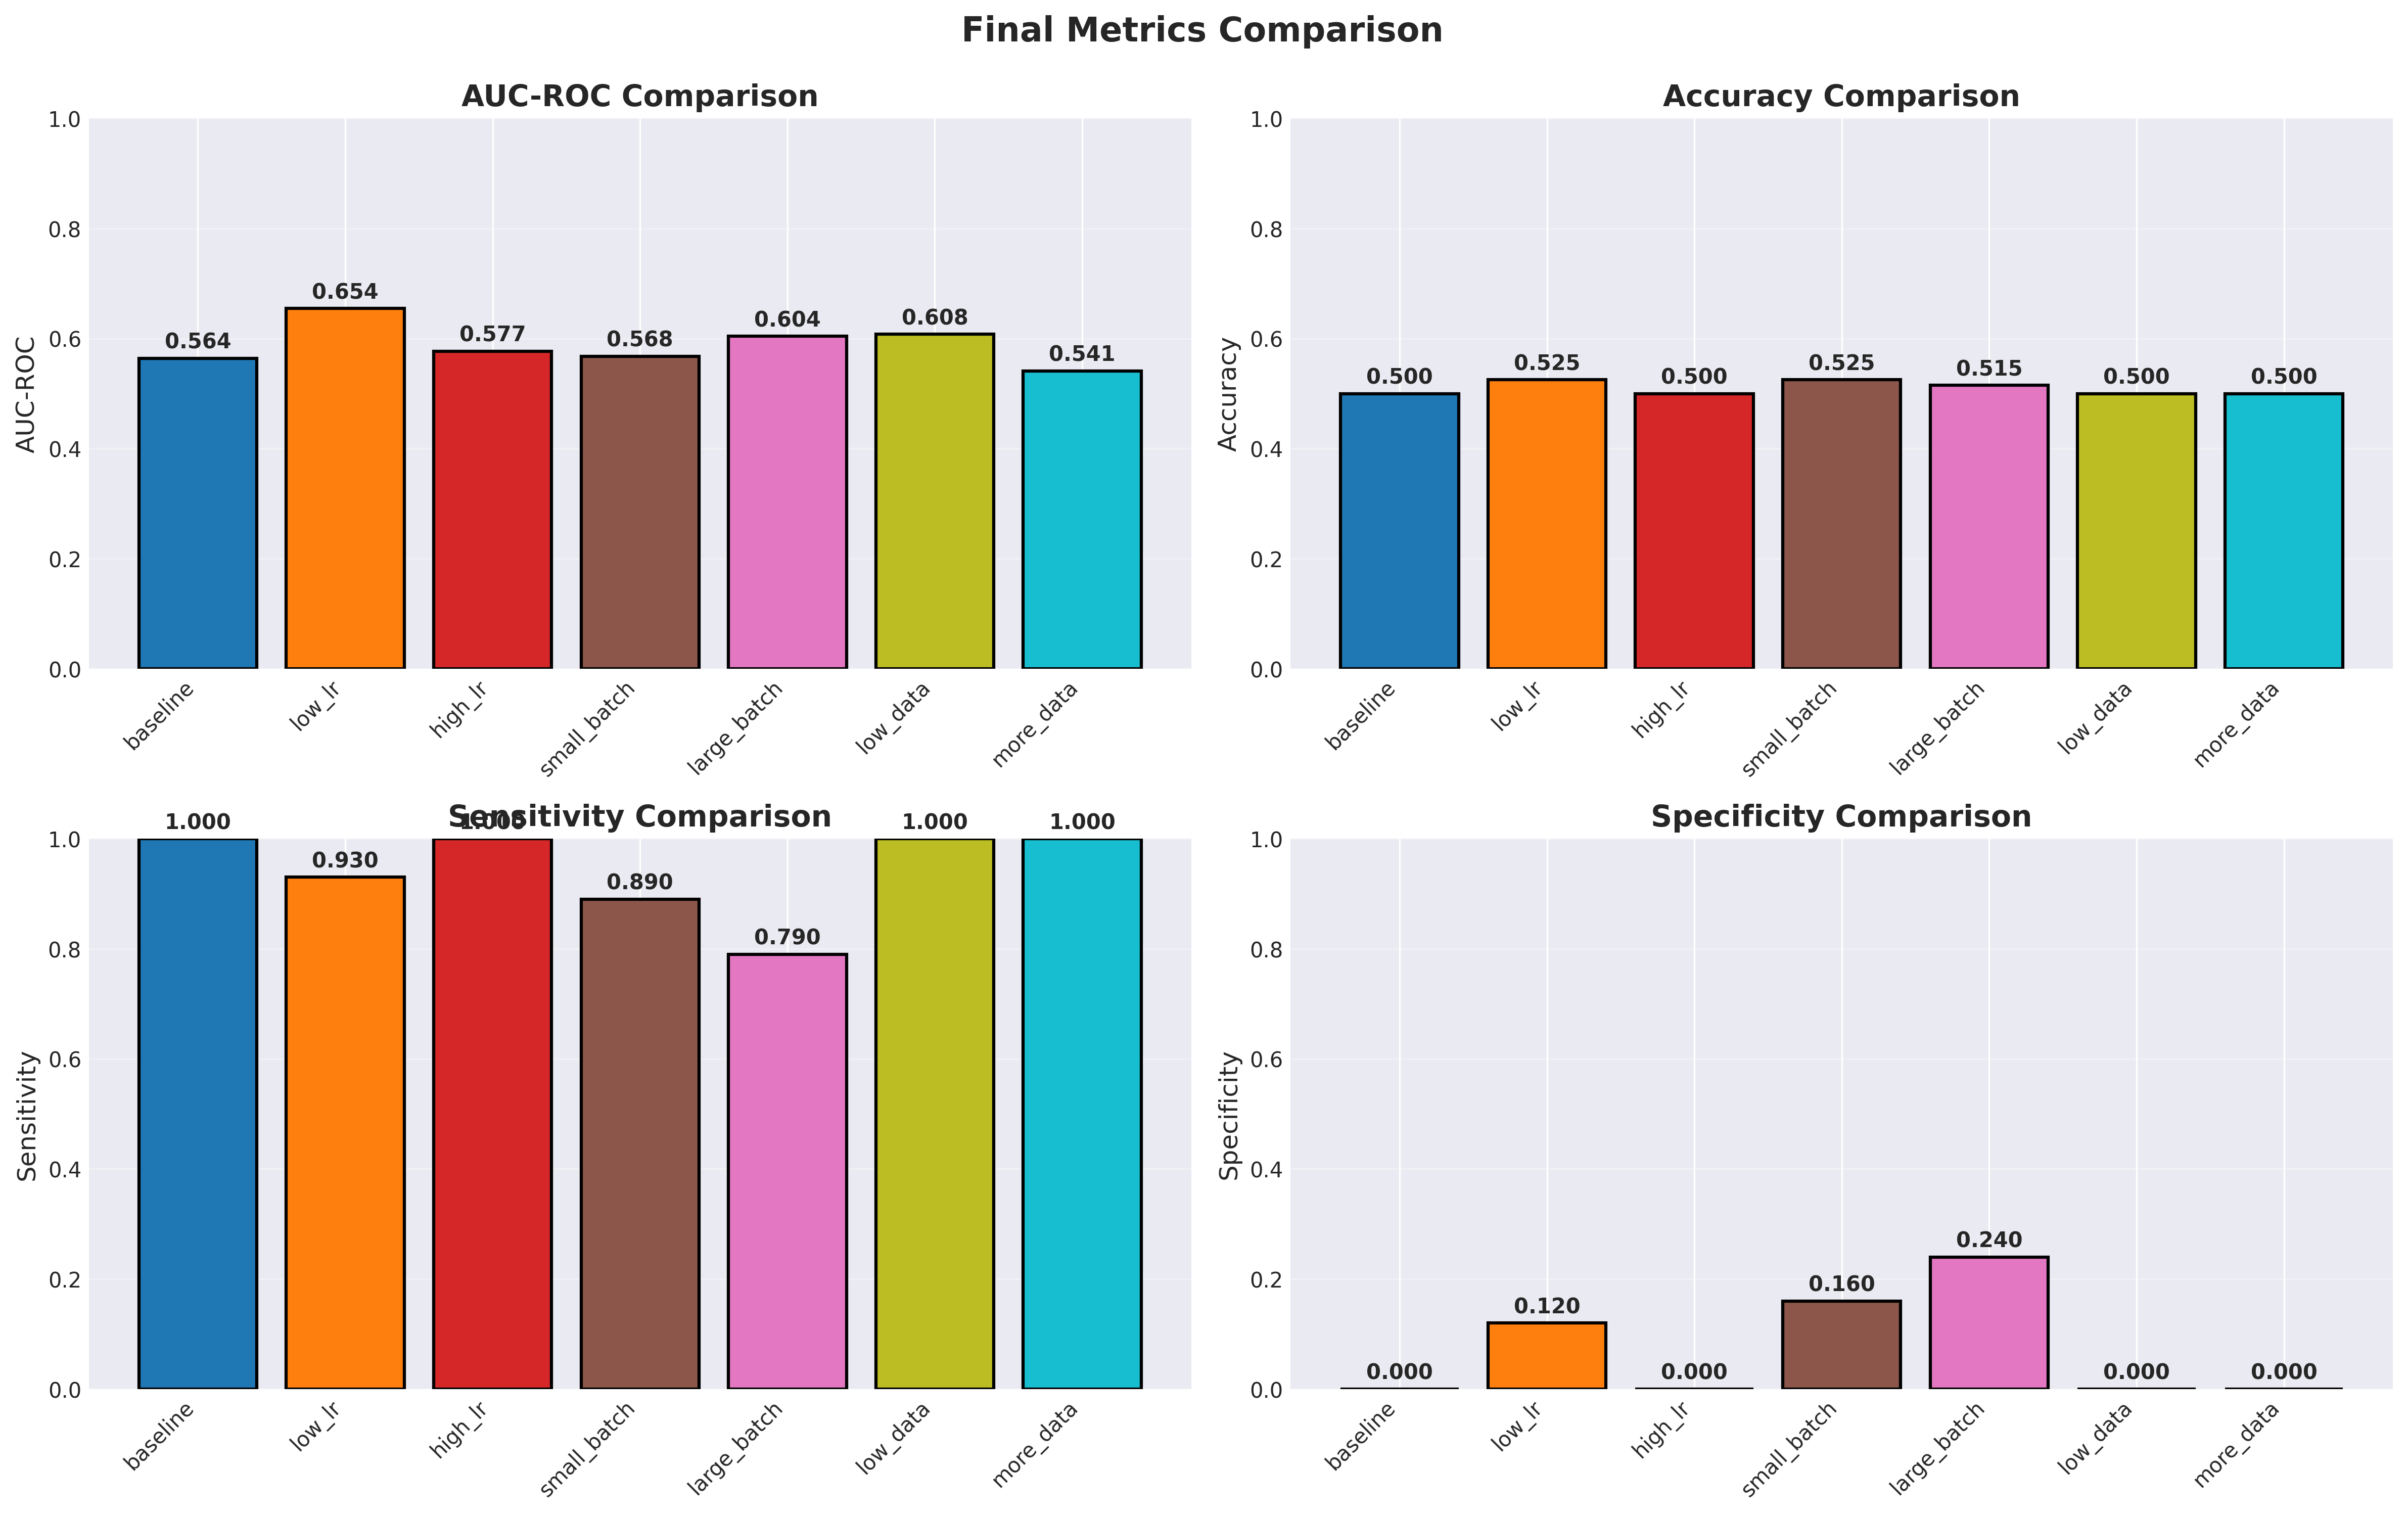
\includegraphics[width=\textwidth]{../results/final_metrics_comparison.png}
\caption{Comparison of final performance metrics across all experimental configurations. The figure shows AUC-ROC and accuracy for each configuration.}
\label{fig:final_metrics}
\end{figure}

\subsection{Effect of the learning rate}
At a fixed training set size of 1000 samples and a constant training budget of 10 epochs, reducing the learning rate from $1 \times 10^{-3}$ to $3 \times 10^{-4}$ resulted in the most substantial improvement in validation AUC-ROC (0.5639 to 0.6545). Increasing the learning rate to $3 \times 10^{-3}$ led to only a limited improvement in performance. Among the hyperparameters explored, the learning rate therefore appears to have the strongest influence on validation performance.

\subsection{Effect of batch size}
When varying the batch size while keeping the learning rate fixed at $1 \times 10^{-3}$ and using 1000 training samples, the configuration with a larger batch size achieved a higher validation AUC-ROC (0.6039) than the small-batch configuration (0.5679). This suggests a moderate benefit from larger batch sizes in this experimental setting.

\subsection{Effect of training dataset size with fixed epochs}
Varying the size of the training dataset (500, 1000, and 2000 samples) while keeping the number of epochs fixed did not result in a consistent improvement in validation AUC-ROC. The \textit{low\_data} configuration, trained on 500 samples, achieved an AUC-ROC of 0.6076, whereas increasing the training set size to 2000 samples (\textit{more\_data}) resulted in a lower AUC-ROC of 0.5409. Under this fixed-epoch protocol, increasing the number of training samples did not translate into improved ranking performance.

\begin{figure}[h]
\centering
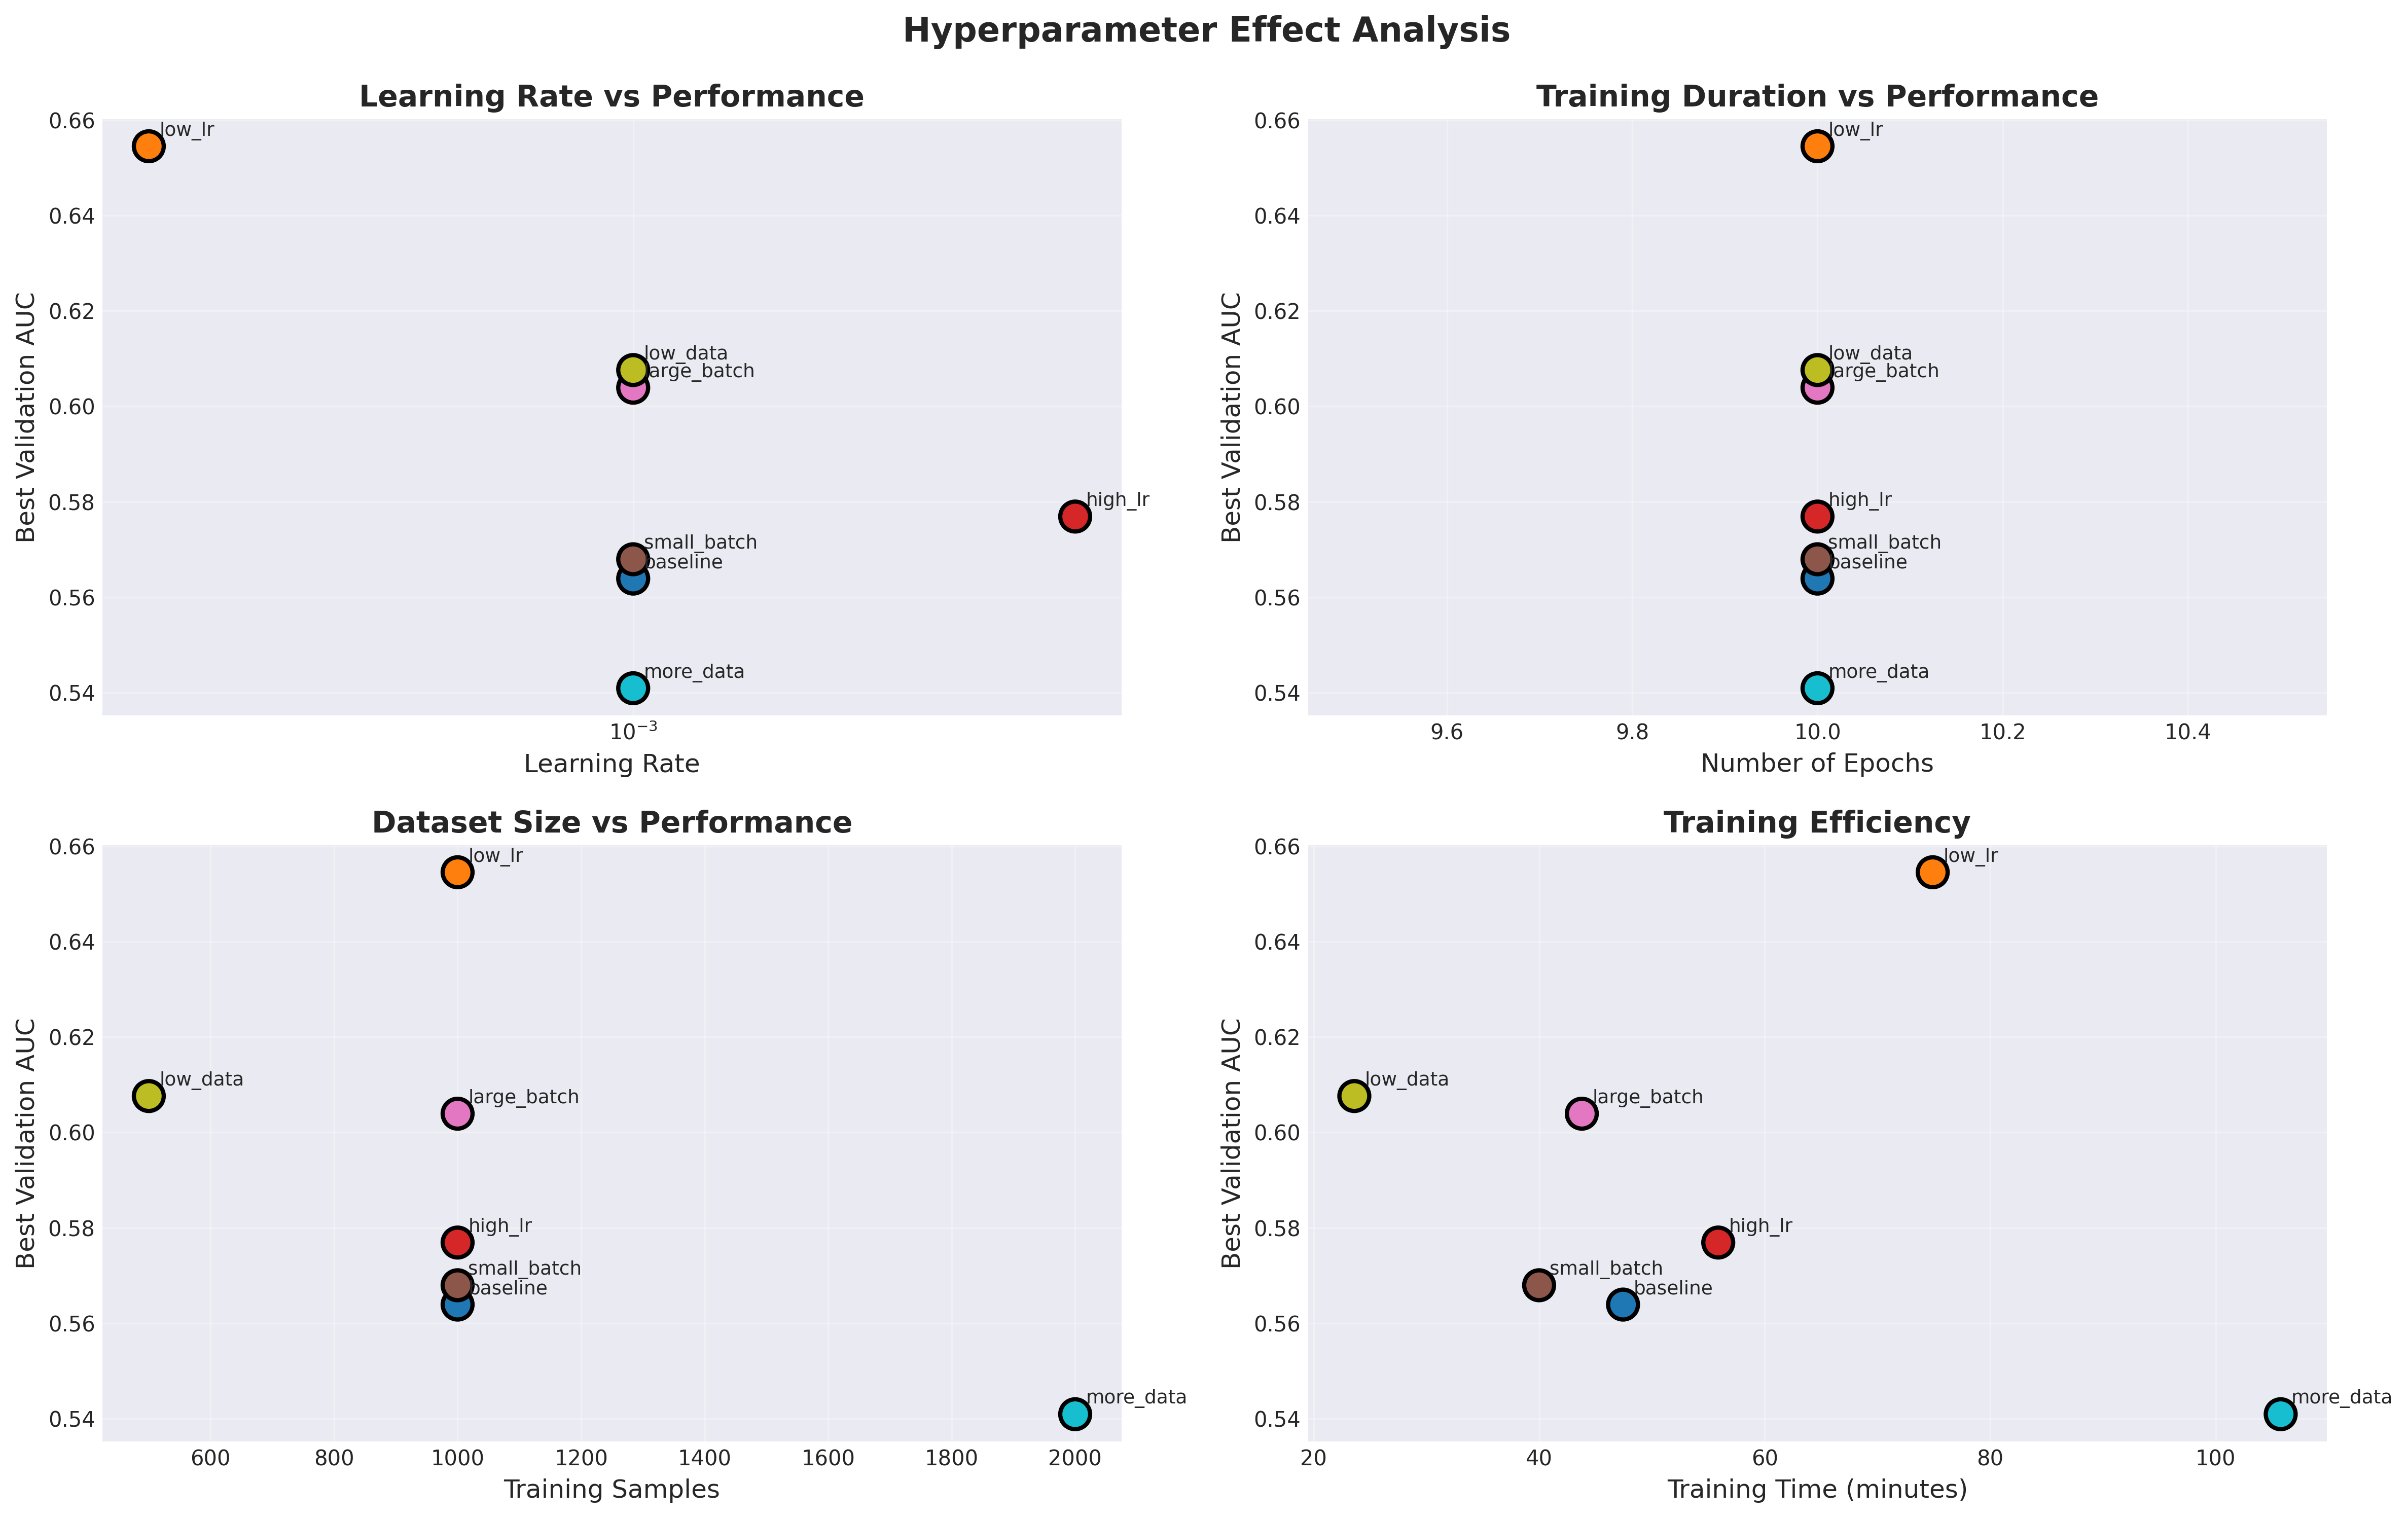
\includegraphics[width=\textwidth]{../results/hyperparameter_analysis.png}
\caption{Hyperparameter effect analysis across experimental configurations. The four panels show the relationship between (top-left) learning rate and validation AUC-ROC, (top-right) training duration and performance, (bottom-left) dataset size and performance, and (bottom-right) training efficiency measured as AUC-ROC per training time.}
\label{fig:hyperparameter_analysis}
\end{figure}

\subsection{Training efficiency and threshold-based metrics}
In terms of computational efficiency, the \textit{low\_data} configuration had the shortest training time (23.6 minutes) and achieved the highest AUC-ROC per minute, making it suitable for rapid experimentation. At the selected decision threshold, the best-performing configuration (\textit{low\_lr}) achieved an accuracy of 0.5250, with a sensitivity of 0.93 and a specificity of 0.12, indicating a strongly recall-oriented operating point.

% Discussion
\section{Discussion}

This study focused on the development and evaluation of a multi-view convolutional neural network based on a ResNet18 backbone for automated abnormality detection in musculoskeletal radiographs. The main objective was to explore whether integrating multiple radiographic projections at the study level could improve the classification of upper extremity X-ray examinations as normal or abnormal. Such an approach is motivated by clinical practice, where radiologists rely on complementary views when interpreting musculoskeletal imaging, and aims to investigate the potential of deep learning as a diagnostic support tool.

The best-performing configuration reached a validation AUC-ROC of 0.6545, indicating a moderate ability to discriminate between normal and abnormal studies. Although this level of performance is not sufficient for direct clinical deployment, it represents a reasonable proof of concept given the constraints of this work. In particular, the model was trained using a limited computational budget and a relatively lightweight architecture. The results suggest that the network was able to combine information from multiple views through the proposed pooling strategy, which is consistent with the intended multi-view design.

From a clinical perspective, the operating characteristics of the model highlight important trade-offs. The configuration with the highest AUC-ROC achieved a high sensitivity of 0.93, meaning that most abnormal cases were correctly identified. This property could be valuable in screening-oriented settings, where minimizing missed abnormalities is a priority. However, this high sensitivity was associated with a very low specificity (0.12), leading to a large number of false positives. As a result, the current model would not be suitable as a standalone diagnostic system.

The observed performance is likely influenced by several methodological and computational limitations. Training was restricted to a subset of 1,000 studies, a fixed budget of 10 epochs, and a ResNet18 architecture in order to accommodate CPU-based training. These constraints may have limited the model’s capacity to fully learn complex and diverse pathological patterns present in the dataset. Despite these limitations, the experiments showed that optimization choices, particularly the learning rate, had a noticeable impact on performance, suggesting that more extensive hyperparameter tuning could lead to further improvements.

Several limitations of this study should be noted. The model was trained and evaluated on a limited subset of the data, which may reduce its generalization to unseen cases. Each configuration was evaluated using a single training run, preventing an assessment of performance variability across different random initializations. In addition, evaluation was restricted to the validation set, and no independent test set was used. Finally, the current approach does not provide interpretability mechanisms to understand which image regions or anatomical structures contribute to the model’s predictions, which is an important aspect for clinical acceptance.

Future work should aim to extend this study by leveraging greater computational resources. This would allow training on the full MURA dataset, increasing the number of training epochs, and exploring more expressive architectures such as deeper convolutional networks or transformer-based models. Incorporating learning rate scheduling, data augmentation, and systematic hyperparameter optimization could also improve performance. Furthermore, adding interpretability methods such as Grad-CAM would help assess whether the model focuses on clinically relevant regions across views. More robust evaluation protocols, including multi-seed experiments, cross-validation, and testing on an independent dataset, would be necessary to better assess generalization and reliability. Ultimately, these extensions would help clarify the practical relevance of multi-view deep learning approaches for musculoskeletal abnormality detection.



\section*{References}

Please number citations consecutively within brackets \cite{b1}. The 
sentence punctuation follows the bracket \cite{b2}. Refer simply to the reference 
number, as in \cite{b3}---do not use ``Ref. \cite{b3}'' or ``reference \cite{b3}'' except at 
the beginning of a sentence: ``Reference \cite{b3} was the first $\ldots$''

Number footnotes separately in superscripts. Place the actual footnote at 
the bottom of the column in which it was cited. Do not put footnotes in the 
abstract or reference list. Use letters for table footnotes.

Unless there are six authors or more give all authors' names; do not use 
``et al.''. Papers that have not been published, even if they have been 
submitted for publication, should be cited as ``unpublished'' \cite{b4}. Papers 
that have been accepted for publication should be cited as ``in press'' \cite{b5}. 
Capitalize only the first word in a paper title, except for proper nouns and 
element symbols.

For papers published in translation journals, please give the English 
citation first, followed by the original foreign-language citation \cite{b6}.

\begin{thebibliography}{00}
\bibitem{b1} G. Eason, B. Noble, and I. N. Sneddon, ``On certain integrals of Lipschitz-Hankel type involving products of Bessel functions,'' Phil. Trans. Roy. Soc. London, vol. A247, pp. 529--551, April 1955.
\bibitem{b2} J. Clerk Maxwell, A Treatise on Electricity and Magnetism, 3rd ed., vol. 2. Oxford: Clarendon, 1892, pp.68--73.
\bibitem{b3} I. S. Jacobs and C. P. Bean, ``Fine particles, thin films and exchange anisotropy,'' in Magnetism, vol. III, G. T. Rado and H. Suhl, Eds. New York: Academic, 1963, pp. 271--350.
\bibitem{b4} K. Elissa, ``Title of paper if known,'' unpublished.
\bibitem{b5} R. Nicole, ``Title of paper with only first word capitalized,'' J. Name Stand. Abbrev., in press.
\bibitem{b6} Y. Yorozu, M. Hirano, K. Oka, and Y. Tagawa, ``Electron spectroscopy studies on magneto-optical media and plastic substrate interface,'' IEEE Transl. J. Magn. Japan, vol. 2, pp. 740--741, August 1987 [Digests 9th Annual Conf. Magnetics Japan, p. 301, 1982].
\bibitem{b7} M. Young, The Technical Writer's Handbook. Mill Valley, CA: University Science, 1989.
\bibitem{b8} D. P. Kingma and M. Welling, ``Auto-encoding variational Bayes,'' 2013, arXiv:1312.6114. [Online]. Available: https://arxiv.org/abs/1312.6114
\bibitem{b9} S. Liu, ``Wi-Fi Energy Detection Testbed (12MTC),'' 2023, gitHub repository. [Online]. Available: https://github.com/liustone99/Wi-Fi-Energy-Detection-Testbed-12MTC
\bibitem{b10} ``Treatment episode data set: discharges (TEDS-D): concatenated, 2006 to 2009.'' U.S. Department of Health and Human Services, Substance Abuse and Mental Health Services Administration, Office of Applied Studies, August, 2013, DOI:10.3886/ICPSR30122.v2
\bibitem{b11} K. Eves and J. Valasek, ``Adaptive control for singularly perturbed systems examples,'' Code Ocean, Aug. 2023. [Online]. Available: https://codeocean.com/capsule/4989235/tree
\end{thebibliography}

\vspace{12pt}
\color{red}
IEEE conference templates contain guidance text for composing and formatting conference papers. Please ensure that all template text is removed from your conference paper prior to submission to the conference. Failure to remove the template text from your paper may result in your paper not being published.

\end{document}
